\documentclass[11pt,a4paper]{article}
\usepackage[utf8]{inputenc}
\usepackage[T1]{fontenc}
\usepackage[margin=2.2cm]{geometry}
\usepackage{graphicx}
\usepackage{booktabs}
\usepackage{multirow}
\usepackage{longtable}
\usepackage{float}
\usepackage{siunitx}
\usepackage[colorlinks=true,linkcolor=black,urlcolor=blue]{hyperref}
\usepackage[inline]{enumitem}
\sisetup{range-phrase=--}
\setlength{\parindent}{0pt}
\setlength{\parskip}{4pt}
\emergencystretch=3em
\title{PRIN 2026: funded units by GSD of the leader}
\author{}
\date{Data of 26/10/2026; 23 of 28 sectors}
\begin{document}
\maketitle
\section{Subsectors 03/CHEM}
\textbf{Purpose.} To describe, for each GSD of the group, the units funded, their money, their ERC sectors, institutions, career levels, gender and partners, using the GSD of the unit leaders.

\textbf{Result.} 56 funded units have a leader whose GSD starts with 03/CHEM (8 coordinators, 48 partners) in 25 projects and 8 ERC sectors; they received 10.78~M~EUR (5.18\% of the budget). The GSD is known for 338 of the 388 unit leaders of these 8 sectors (leaders of research bodies and of institutions that are not universities are not in the directory). The staff of the directory is known by CUN area, not by GSD, so nothing is divided by the staff of a GSD.

\begin{table}[H]
\centering
\footnotesize
\begin{tabular}{lrrrrrrrr}
\toprule
GSD & Units & PI & Projects & Institutions & ERC sectors & k EUR & Share \% & k EUR/unit \\
\midrule
CHEM-01 & 3 & 0 & 3 & 3 & 3 & 533 & 0.26 & 178 \\
CHEM-02 & 10 & 2 & 7 & 8 & 4 & 1962 & 0.94 & 196 \\
CHEM-03 & 13 & 2 & 5 & 10 & 1 & 2632 & 1.26 & 202 \\
CHEM-04 & 4 & 0 & 4 & 4 & 3 & 866 & 0.42 & 217 \\
CHEM-05 & 19 & 4 & 7 & 16 & 3 & 3538 & 1.70 & 186 \\
CHEM-06 & 1 & 0 & 1 & 1 & 1 & 234 & 0.11 & 234 \\
CHEM-07 & 6 & 0 & 5 & 6 & 2 & 1019 & 0.49 & 170 \\
All & 56 & 8 & 25 & 31 & 8 & 10783 & 5.18 & 193 \\
\bottomrule
\end{tabular}
\end{table}
\begin{table}[H]
\centering
\footnotesize
\begin{tabular}{lrrrrrr}
\toprule
GSD & Women \% & PI under 40 & PO & PA & RTD & RU \\
\midrule
CHEM-01 & 67 & 0 & 0 & 3 & 0 & 0 \\
CHEM-02 & 30 & 0 & 5 & 4 & 1 & 0 \\
CHEM-03 & 31 & 0 & 7 & 6 & 0 & 0 \\
CHEM-04 & 50 & 0 & 3 & 1 & 0 & 0 \\
CHEM-05 & 58 & 1 & 6 & 11 & 2 & 0 \\
CHEM-06 & 100 & 0 & 1 & 0 & 0 & 0 \\
CHEM-07 & 0 & 0 & 3 & 2 & 1 & 0 \\
All & 41 & 1 & 25 & 27 & 4 & 0 \\
\bottomrule
\end{tabular}
\end{table}
{\footnotesize Units: funded units whose leader's GSD is the row's; PI: of these, coordinators; Institutions and ERC sectors: distinct ones with such a unit; Share: of the total budget; Women: among these leaders; PI under 40: units led by a PI under 40; PO, PA, RTD, RU: full professors, associate professors, fixed-term and permanent researchers.}

\begin{table}[H]
\centering
\footnotesize
\begin{tabular}{lrrrr}
\toprule
Sub-sector (SSD) & Units & PI & k EUR & Share \% \\
\midrule
CHEM-01/A & 2 & 0 & 335 & 0.16 \\
CHEM-01/B & 1 & 0 & 198 & 0.09 \\
CHEM-02/A & 10 & 2 & 1962 & 0.94 \\
CHEM-03/A & 13 & 2 & 2632 & 1.26 \\
CHEM-04/A & 4 & 0 & 866 & 0.42 \\
CHEM-05/A & 19 & 4 & 3538 & 1.70 \\
CHEM-06/A & 1 & 0 & 234 & 0.11 \\
CHEM-07/A & 6 & 0 & 1019 & 0.49 \\
\bottomrule
\end{tabular}
\end{table}
\begin{figure}[H]
\centering
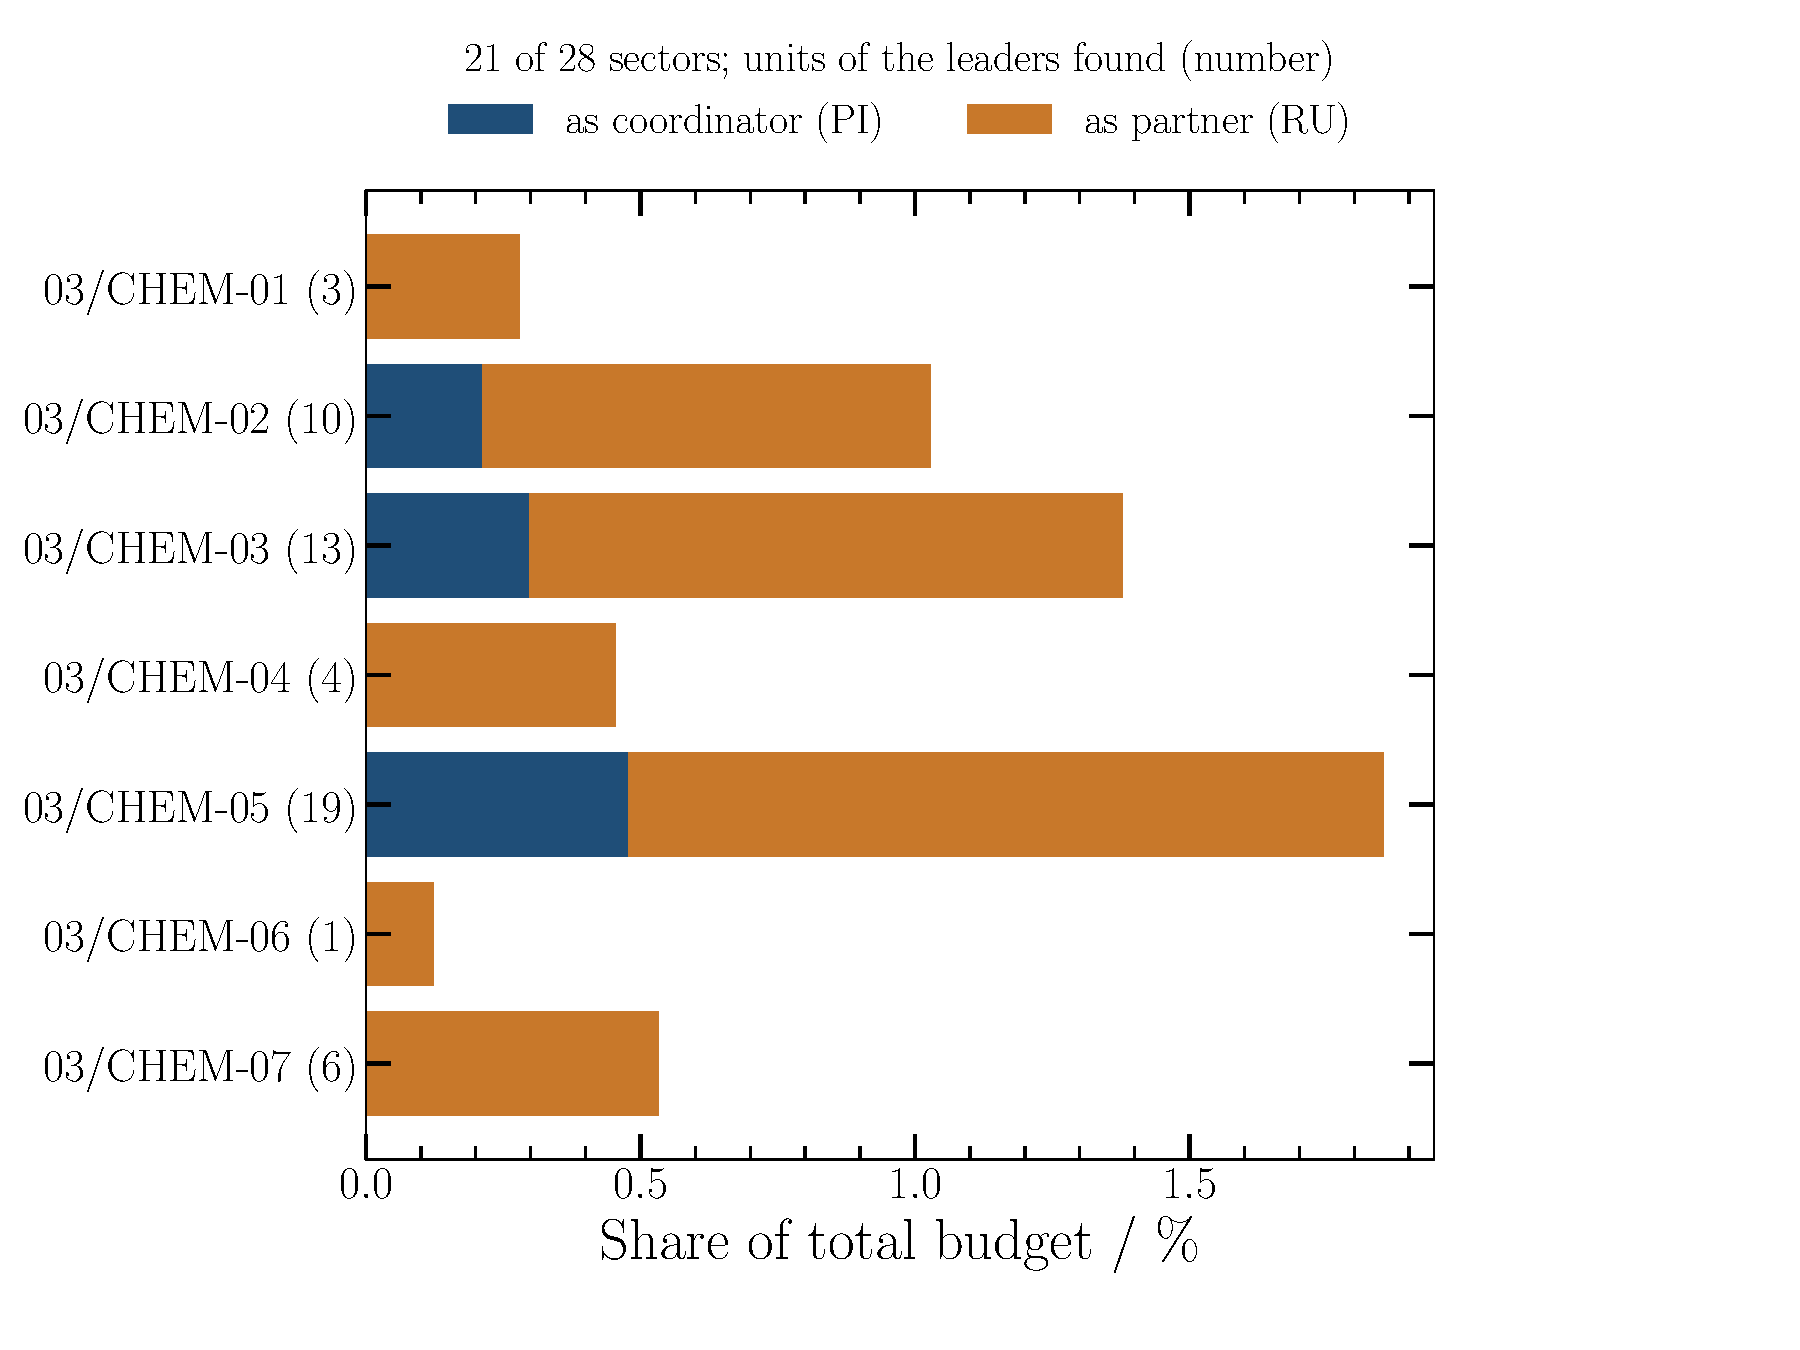
\includegraphics[width=0.75\textwidth]{../prin_out/figures/focus_03_chem_money.pdf}
\caption{Money of the units by GSD of the leader, in percent of the total budget; in brackets the number of units.}
\end{figure}
\begin{figure}[H]
\centering
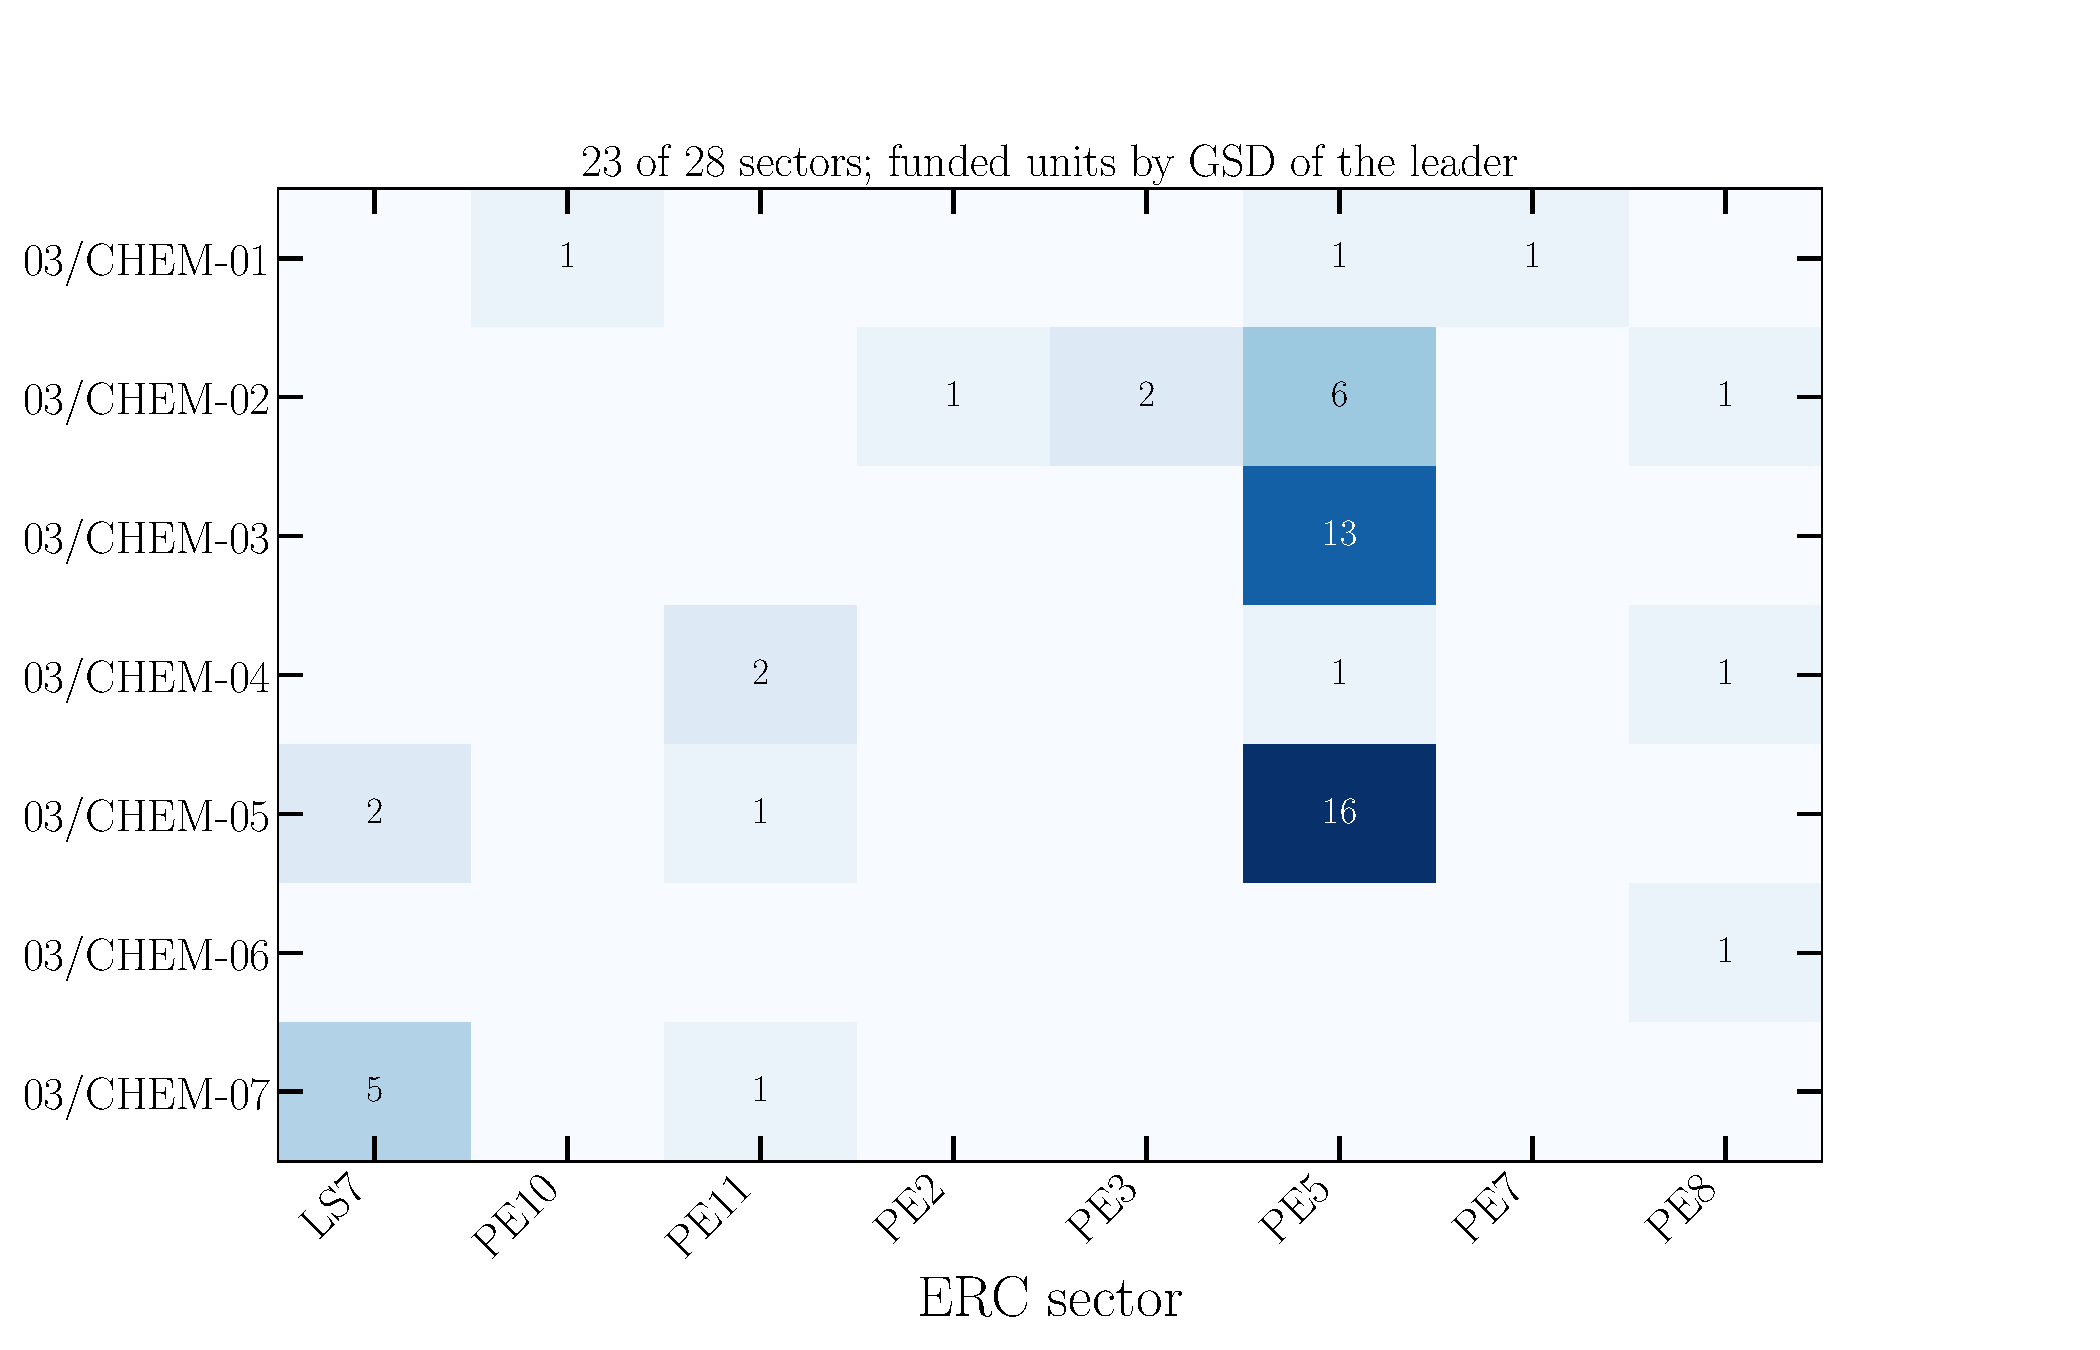
\includegraphics[width=0.8\textwidth]{../prin_out/figures/focus_03_chem_sectors.pdf}
\caption{Number of funded units by GSD of the leader and ERC sector.}
\end{figure}
\begin{figure}[H]
\centering
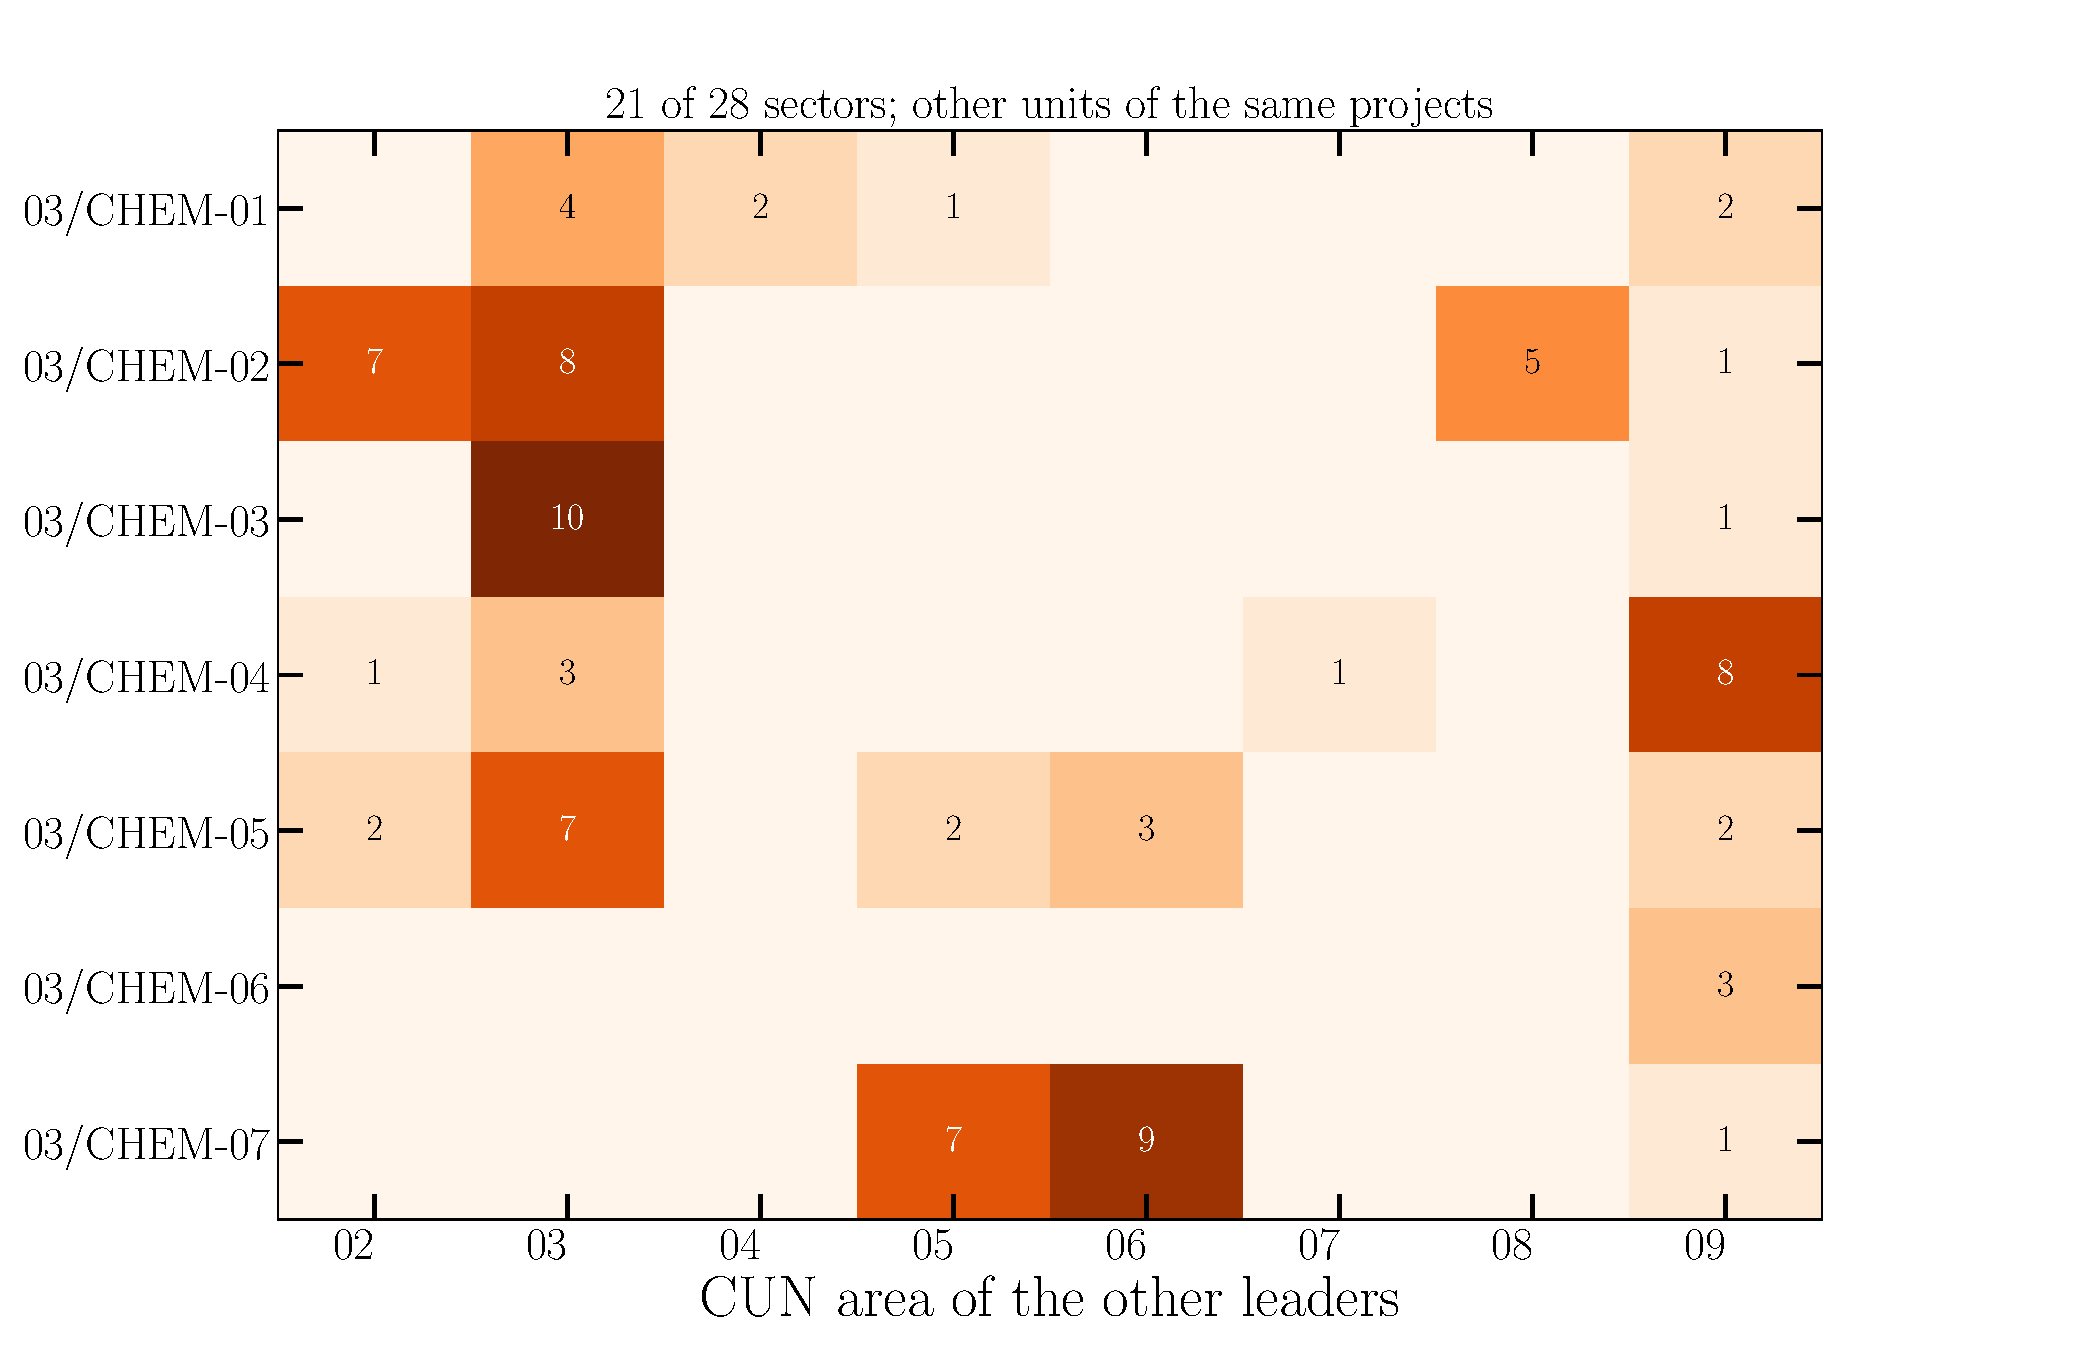
\includegraphics[width=0.85\textwidth]{../prin_out/figures/focus_03_chem_partners.pdf}
\caption{Units of the projects that have a unit of the GSD, by CUN area of their leader (units of the GSD itself excluded; leaders whose GSD was not found are not counted). Areas: 02 Physics, 03 Chemistry, 04 Earth sciences, 05 Biology, 06 Medicine, 07 Agriculture, veterinary, 08 Civil eng., architecture, 09 Industrial, information eng.}
\end{figure}

\clearpage
\subsection{GSD 03/CHEM-01}
\textbf{Purpose.} To list the units of one GSD by ERC sector and by institution.

\textbf{Result.} 3 units (0 coordinators) in 3 projects, at 3 institutions, in 3 ERC sectors, 0.53~M~EUR (0.26\% of the budget, 178 k EUR per unit); women among the leaders 2 of 3; career levels PO 0, PA 3, RTD 0, RU 0; PIs under 40: 0. The projects have 12 other units, of which 9 have a leader with a known GSD: Chemistry 4, Earth sciences 2, Industrial, information eng. 2, Biology 1. Sub-sectors: CHEM-01/A 2 and CHEM-01/B 1.

{\footnotesize
\begin{longtable}{lrrr}
\toprule
ERC sector & Units & PI & k EUR \\
\midrule
\endhead
PE10 & 1 & 0 & 198 \\
PE5 & 1 & 0 & 176 \\
PE7 & 1 & 0 & 159 \\
\midrule
Total & 3 & 0 & 533 \\
\bottomrule
\end{longtable}
}
{\footnotesize
\begin{longtable}{lrr}
\toprule
Institution & Units & k EUR \\
\midrule
\endhead
Genova & 1 & 198 \\
Padova & 1 & 176 \\
Tor Vergata & 1 & 159 \\
\bottomrule
\end{longtable}
}

\clearpage
\subsection{GSD 03/CHEM-02}
\textbf{Purpose.} To list the units of one GSD by ERC sector and by institution.

\textbf{Result.} 10 units (2 coordinators) in 7 projects, at 8 institutions, in 4 ERC sectors, 1.96~M~EUR (0.94\% of the budget, 196 k EUR per unit); women among the leaders 3 of 10; career levels PO 5, PA 4, RTD 1, RU 0; PIs under 40: 0. The projects have 27 other units, of which 21 have a leader with a known GSD: Chemistry 8, Physics 7, Civil eng., architecture 5, Industrial, information eng. 1.

{\footnotesize
\begin{longtable}{lrrr}
\toprule
ERC sector & Units & PI & k EUR \\
\midrule
\endhead
PE2 & 1 & 0 & 291 \\
PE3 & 2 & 0 & 349 \\
PE5 & 6 & 2 & 1141 \\
PE8 & 1 & 0 & 181 \\
\midrule
Total & 10 & 2 & 1962 \\
\bottomrule
\end{longtable}
}
{\footnotesize
\begin{longtable}{lrr}
\toprule
Institution & Units & k EUR \\
\midrule
\endhead
Firenze & 2 & 513 \\
Torino & 2 & 342 \\
Politecnico di Torino & 1 & 195 \\
Federico II & 1 & 195 \\
Padova & 1 & 191 \\
Salento & 1 & 189 \\
Calabria & 1 & 181 \\
Perugia & 1 & 156 \\
\bottomrule
\end{longtable}
}

\clearpage
\subsection{GSD 03/CHEM-03}
\textbf{Purpose.} To list the units of one GSD by ERC sector and by institution.

\textbf{Result.} 13 units (2 coordinators) in 5 projects, at 10 institutions, in 1 ERC sectors, 2.63~M~EUR (1.26\% of the budget, 202 k EUR per unit); women among the leaders 4 of 13; career levels PO 7, PA 6, RTD 0, RU 0; PIs under 40: 0. The projects have 13 other units, of which 11 have a leader with a known GSD: Chemistry 10, Industrial, information eng. 1.

{\footnotesize
\begin{longtable}{lrrr}
\toprule
ERC sector & Units & PI & k EUR \\
\midrule
\endhead
PE5 & 13 & 2 & 2632 \\
\midrule
Total & 13 & 2 & 2632 \\
\bottomrule
\end{longtable}
}
{\footnotesize
\begin{longtable}{lrr}
\toprule
Institution & Units & k EUR \\
\midrule
\endhead
Bologna & 2 & 570 \\
Firenze & 2 & 400 \\
Modena e Reggio Emilia & 2 & 375 \\
Bari Aldo Moro & 1 & 229 \\
Vanvitelli & 1 & 226 \\
Parma & 1 & 176 \\
Palermo & 1 & 174 \\
Perugia & 1 & 166 \\
Milano Statale & 1 & 164 \\
Magna Graecia & 1 & 152 \\
\bottomrule
\end{longtable}
}

\clearpage
\subsection{GSD 03/CHEM-04}
\textbf{Purpose.} To list the units of one GSD by ERC sector and by institution.

\textbf{Result.} 4 units (0 coordinators) in 4 projects, at 4 institutions, in 3 ERC sectors, 0.87~M~EUR (0.42\% of the budget, 217 k EUR per unit); women among the leaders 2 of 4; career levels PO 3, PA 1, RTD 0, RU 0; PIs under 40: 0. The projects have 16 other units, of which 13 have a leader with a known GSD: Industrial, information eng. 8, Chemistry 3, Physics 1, Agriculture, veterinary 1.

{\footnotesize
\begin{longtable}{lrrr}
\toprule
ERC sector & Units & PI & k EUR \\
\midrule
\endhead
PE11 & 2 & 0 & 462 \\
PE5 & 1 & 0 & 173 \\
PE8 & 1 & 0 & 232 \\
\midrule
Total & 4 & 0 & 866 \\
\bottomrule
\end{longtable}
}
{\footnotesize
\begin{longtable}{lrr}
\toprule
Institution & Units & k EUR \\
\midrule
\endhead
Genova & 1 & 268 \\
Bologna & 1 & 232 \\
Sassari & 1 & 194 \\
Milano-Bicocca & 1 & 173 \\
\bottomrule
\end{longtable}
}

\clearpage
\subsection{GSD 03/CHEM-05}
\textbf{Purpose.} To list the units of one GSD by ERC sector and by institution.

\textbf{Result.} 19 units (4 coordinators) in 7 projects, at 16 institutions, in 3 ERC sectors, 3.54~M~EUR (1.70\% of the budget, 186 k EUR per unit); women among the leaders 11 of 19; career levels PO 6, PA 11, RTD 2, RU 0; PIs under 40: 1. The projects have 20 other units, of which 16 have a leader with a known GSD: Chemistry 7, Medicine 3, Physics 2, Biology 2, Industrial, information eng. 2.

{\footnotesize
\begin{longtable}{lrrr}
\toprule
ERC sector & Units & PI & k EUR \\
\midrule
\endhead
LS7 & 2 & 0 & 325 \\
PE11 & 1 & 0 & 172 \\
PE5 & 16 & 4 & 3041 \\
\midrule
Total & 19 & 4 & 3538 \\
\bottomrule
\end{longtable}
}
{\footnotesize
\begin{longtable}{lrr}
\toprule
Institution & Units & k EUR \\
\midrule
\endhead
Federico II & 2 & 410 \\
Padova & 2 & 372 \\
Milano Statale & 2 & 361 \\
Piemonte Orientale & 1 & 294 \\
Firenze & 1 & 197 \\
Milano-Bicocca & 1 & 197 \\
Parma & 1 & 191 \\
Siena & 1 & 173 \\
Torino & 1 & 173 \\
Basilicata & 1 & 173 \\
Camerino & 1 & 172 \\
Genova & 1 & 166 \\
Pavia & 1 & 166 \\
Tuscia & 1 & 166 \\
Bari Aldo Moro & 1 & 165 \\
Sannio & 1 & 163 \\
\bottomrule
\end{longtable}
}

\clearpage
\subsection{GSD 03/CHEM-06}
\textbf{Purpose.} To list the units of one GSD by ERC sector and by institution.

\textbf{Result.} 1 units (0 coordinators) in 1 projects, at 1 institutions, in 1 ERC sectors, 0.23~M~EUR (0.11\% of the budget, 234 k EUR per unit); women among the leaders 1 of 1; career levels PO 1, PA 0, RTD 0, RU 0; PIs under 40: 0. The projects have 4 other units, of which 3 have a leader with a known GSD: Industrial, information eng. 3.

{\footnotesize
\begin{longtable}{lrrr}
\toprule
ERC sector & Units & PI & k EUR \\
\midrule
\endhead
PE8 & 1 & 0 & 234 \\
\midrule
Total & 1 & 0 & 234 \\
\bottomrule
\end{longtable}
}
{\footnotesize
\begin{longtable}{lrr}
\toprule
Institution & Units & k EUR \\
\midrule
\endhead
Messina & 1 & 234 \\
\bottomrule
\end{longtable}
}

\clearpage
\subsection{GSD 03/CHEM-07}
\textbf{Purpose.} To list the units of one GSD by ERC sector and by institution.

\textbf{Result.} 6 units (0 coordinators) in 5 projects, at 6 institutions, in 2 ERC sectors, 1.02~M~EUR (0.49\% of the budget, 170 k EUR per unit); women among the leaders 0 of 6; career levels PO 3, PA 2, RTD 1, RU 0; PIs under 40: 0. The projects have 21 other units, of which 17 have a leader with a known GSD: Medicine 9, Biology 7, Industrial, information eng. 1.

{\footnotesize
\begin{longtable}{lrrr}
\toprule
ERC sector & Units & PI & k EUR \\
\midrule
\endhead
LS7 & 5 & 0 & 885 \\
PE11 & 1 & 0 & 134 \\
\midrule
Total & 6 & 0 & 1019 \\
\bottomrule
\end{longtable}
}
{\footnotesize
\begin{longtable}{lrr}
\toprule
Institution & Units & k EUR \\
\midrule
\endhead
Sapienza & 1 & 215 \\
Parma & 1 & 182 \\
Salerno & 1 & 176 \\
Vanvitelli & 1 & 176 \\
Roma Tre & 1 & 135 \\
Tor Vergata & 1 & 134 \\
\bottomrule
\end{longtable}
}

\end{document}
